\chapter{Results}


\section{G3BP1 tethering affects mRNA dynamics}

Proteins of the G3BP RNA-binding family are key components of SGs.
In mammals, G3BP1 (and its paralog G3BP2) were reported to be essential in nucleating the formation of SGs \cite{kedersha_g3bp-caprin1-usp10_2016}.
SGs can not only be induced by stress (e.g. sodium arsenite) but also by the overexpression of G3BPs \cite{tourriere_rasgap-associated_2003}.
In addition, a recent imaging-based study Markmiller et al. \cite{markmiller_context-dependent_2018} showed that "many well-characterized SG proteins (e.g., G3BP1, TIA1, CAPRIN1, PABPC1, FMR1, and ATXN2) were identified as highly significant interactors".
This finding might suggest the formation of an mRNP complex containing SG proteins allowing for a rapid assembly.

The exact role of G3BPs in SG assembly as well as in unstressed cells is still largely unknown.
As reviewed in Alam and Kenedy \cite{alam_rasputin_2019} various functions have been attributed to this protein family.
These range from transcript destabilization and repression to the polar opposite in transcript stabilization.
Furthermore, G3BP's also showed effects on transcript localization and sequestration to virus-induced foci.
The only consensus is G3BP's involvement in mRNA translational control.
The subsequent experiments attempt to clarify this disunity by analyzing G3BP1's effect on mRNA transcripts at a single-molecule level.
For this reason, I designed an assay to tether G3BP1 and reporter mRNAs together and thereby promoting mRNA accumulation in SGs.

\begin{figure}[b!]
    \centering
    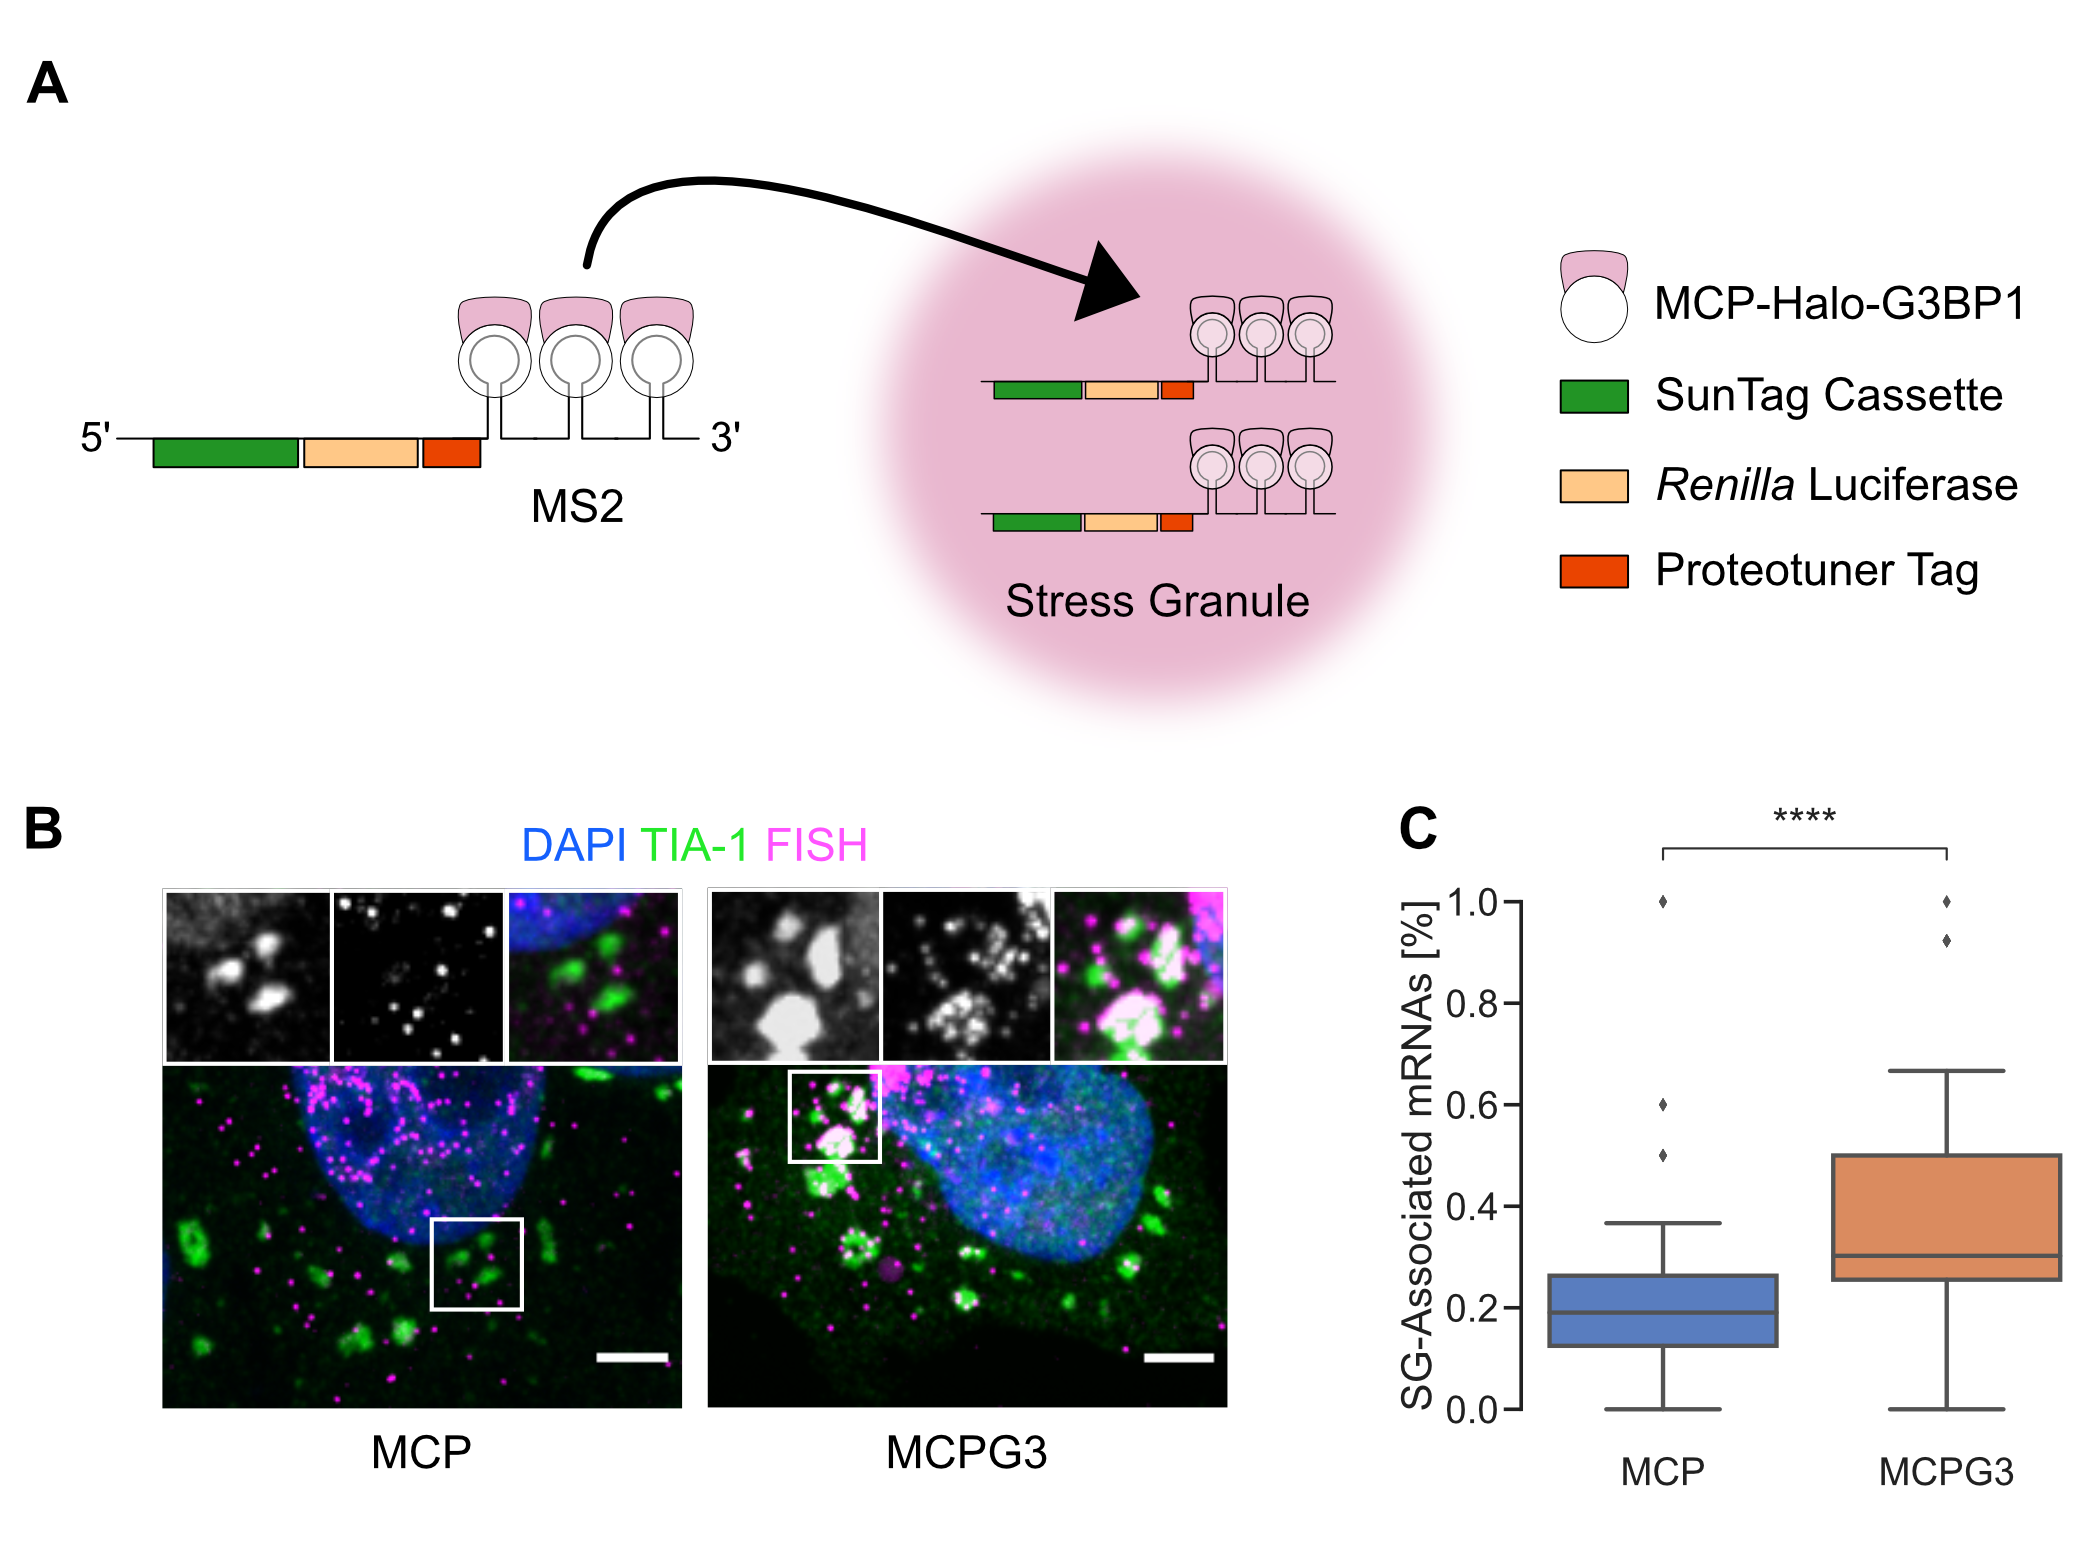
\includegraphics[width=\linewidth]{images/figure2}
    \caption{\textbf{Design of MCP-G3BP1.}
        (A) Schematic depiction of MCP-G3BP1 function.
        (B) Representative fluorescence images of the SG marker
            TIA-1 and the tethered RNAs.
            To induce SGs, cells were treated with 1 mM/ml sodium arsenite for 1 hour.
            Pannels show TIA-1, FISH, Merge respectively.
            Scale bars, 10 \textmu m.
        (C) Quantification of the mRNA recruitment to SGs.
            Number of cells quantified (left to right): 27, 21. 
    }
    \label{fig:mcp_images}
\end{figure}

This study focussed on one reporter RNA containing a SunTag cassette, the gene encoding for \textit{Renilla} luciferase and MS2 stem-loops (Figure \ref{fig:mcp_images}A).
These stem-loops are structural motifs derived from phages and can be specifically recognized by a bacteriophage MS2 coat protein (MCP).
G3BP1 was fused to MCP (abbreviated as MCPG3) in an attempt to promote mRNA recruitment to SGs.
The construct was validated by FISH against the reporter RNA followed by immunofluorescence for the endogenous SG marker TIA-1 \cite{kedersha_rna-binding_1999} (Figure \ref{fig:mcp_images}B).
SGs were induced by sodium arsenite treatment (1 mM/ml for 1 hour).
As a control, an identical construct only lacking G3BP1 fusion was used.
Both by visual inspection as well as by mRNA quantification (Figure \ref{fig:mcp_images}C), a significant difference in SG association can be seen.
MCPG3 shows an approximately two-fold increase in SG associated mRNAs compared to the control.
Taken together, fusing G3BP1 to MCP seems to be a reliable way to recruit functional G3BP1 to the local vicinity of mRNAs and thereby promote localization to SGs.


\subsection{Reporter expression is impacted by G3BP1} \label{mcp_luciferase}

Having proven that G3BP1 can be recruited to mRNAs, I wanted to investigate the effect on translational activity. \textit{Renilla} luciferase assays are used to measure reporter expression on a global level.
As G3BP1 was shown to be involved in stress-induced events as well as in unstressed conditions, the luciferase activity at multiple time points in unstressed cells as well as in cells recovering from oxidative stress was measured.

\begin{figure}[t!]
    \centering
    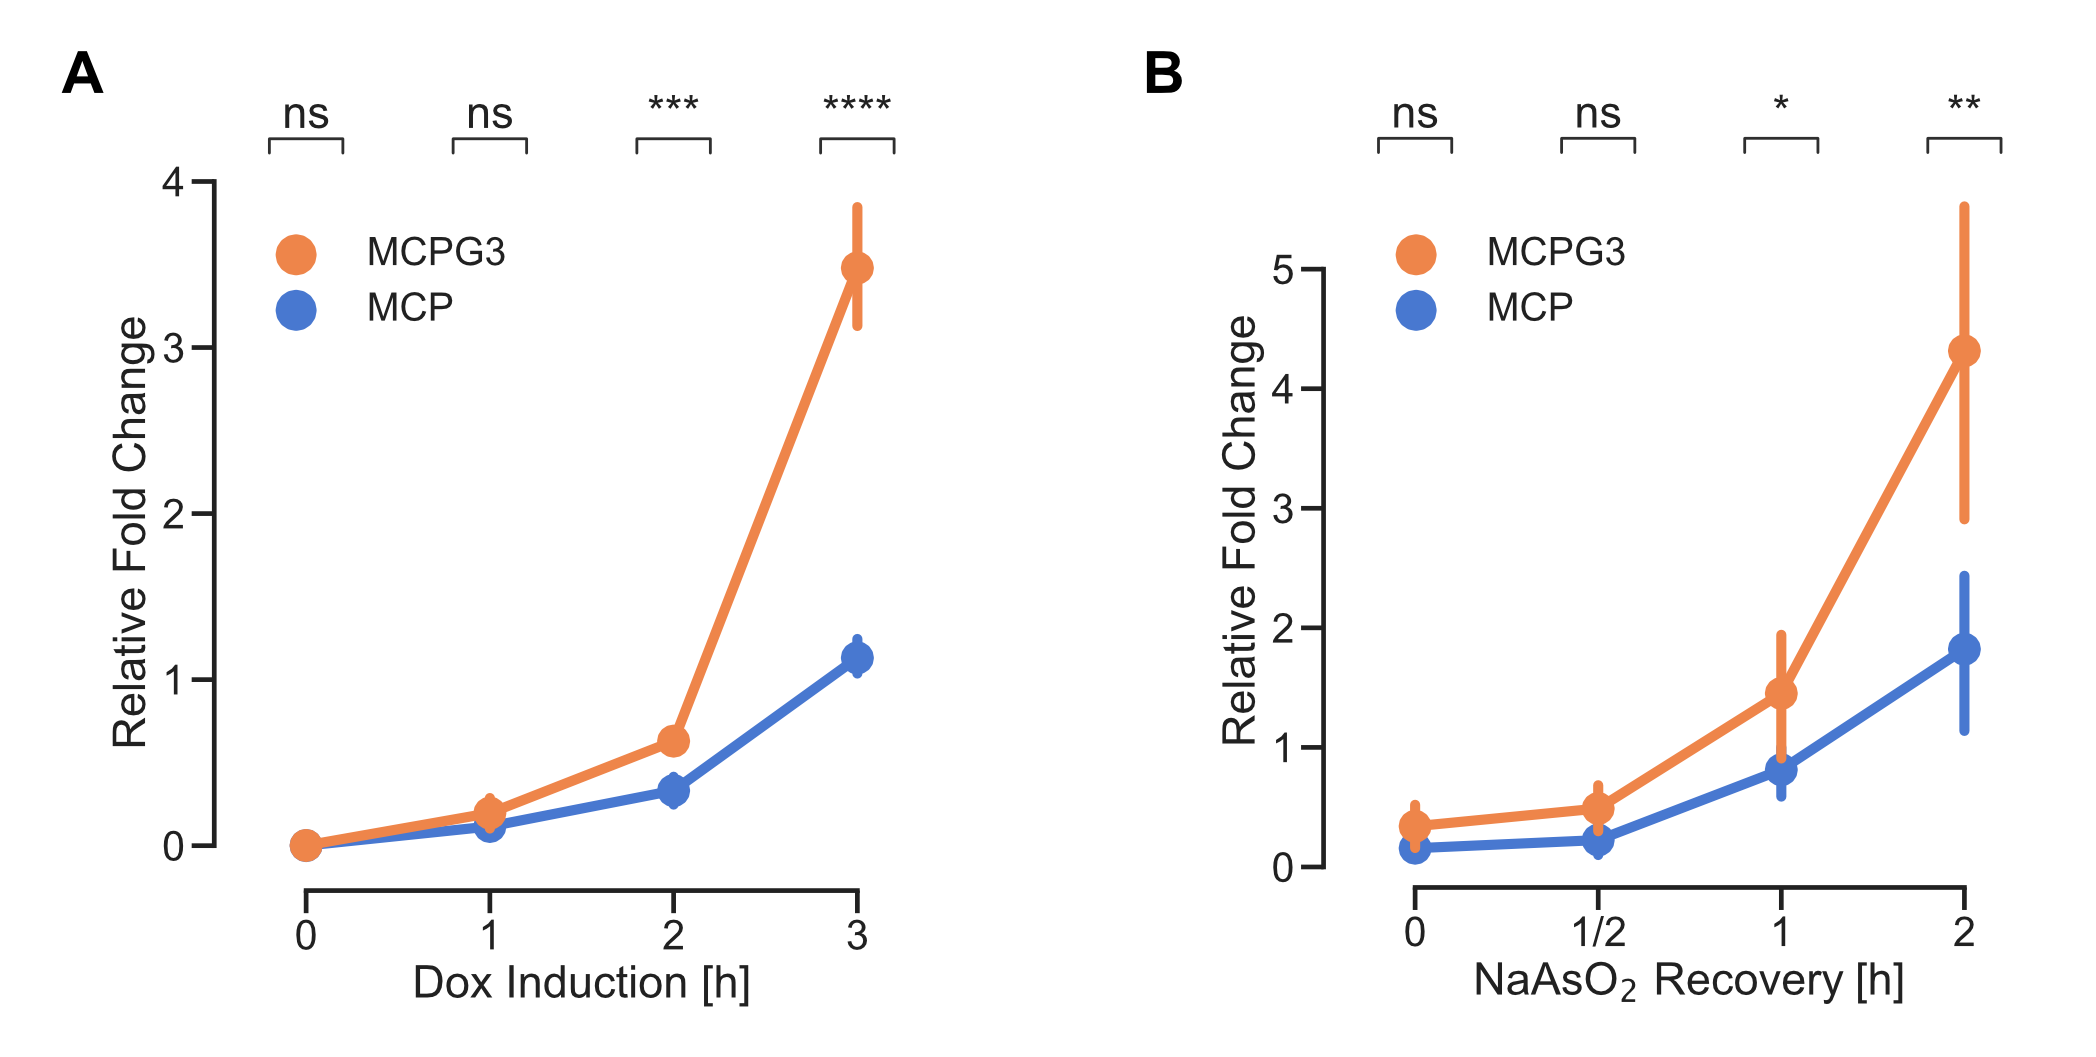
\includegraphics[width=\linewidth]{images/figure3}
    \caption{\textbf{G3BP1 tethering increases global translational activity.}
        (A) Luciferase assays at different time points during induction.
        (B) Sodium arsenite stress recovery time points after induction.
            Cells were induced for 3 hours and stressed with sodium arsenite (1 mM/ml) in the last hour.
            Time point capture started immediately after washing out stressor.
        (A and B) Data normalized to the 3 hour induction condition of MCP.     
    }
    \label{fig:mcp_luciferase}
\end{figure}

The recruitment of G3BP1 to mRNAs showed a significant increase in luciferase readings when looking at the time-points for induction (Figure \ref{fig:mcp_luciferase}A).
This suggests that the presence of G3BP1 might promote protein synthesis.
Comparing both constructs during stress recovery, one can observe a slightly less significant but still noticeable increase in luciferase activity for MCPG3 expressing cells (Figure \ref{fig:mcp_luciferase}B).
Interestingly, the largest effects are at later time points and during non-stress conditions while not being immediately after stress recovery.
This suggests a lesser involvement of G3BP1 on translational activity during stress.
SGs have been observed to persist between a few minutes to hours \cite{chen_relationships_2017}.
This correlates with the time when an increase in luciferase activity can be observed again.


\subsection{G3BP1 does not alter mRNA translation}\label{mcp_suntag}

The observed differences in luciferase activity described in Section \ref{mcp_luciferase} can result from various causes.
These differences in reporter protein synthesis levels could arise from an increase in translational activity of mRNAs or an increase in mRNA stability.
The translation site imaging method SunTag (see Section \ref{translation_site_imaging}) can be used to address this option.

In SunTag, the fluorescence intensity is a direct measure of translation rate.
Therefore, to analyze the translation activity of MCPG3-bound mRNAs, the track intensity was quantified.
Track intensity refers to the average fluorescence intensity over the entire track duration.

During stress conditions, most mRNAs get translationally silenced (reviewed in Holcik and Sonenberg \cite{holcik_translational_2005}).
To image translation sites despite this silencing, images were acquired 15 to 30 minutes after removing the stressor.

Image-level SunTag track intensities in cells expressing MCPG3 or control MCP (Figure \ref{fig:mcp_suntag}A).
Both conditions show similar fluorescence intensities suggesting G3BP1 does not have a major effect on mRNA translation rates.
The lower readings of fluorescent intensity in the stress condition can be explained by translational silencing during stress which was not fully recovered.
Similarly, the grouping of SunTag tracks into segmented cells shows comparable mean intensities in cells expressing MCPG3 or control MCP.
Equivalently to the image-level analysis, cellular intensities (Figure \ref{fig:mcp_suntag}B) do not yield different results.
Similarly, the average intensity of all tracks per cell does not appear to be affected by G3BP1 fusion.

Lastly, global translation can also increase by a higher number of translating transcripts per cell.
However, as is evident from Figure \ref{fig:mcp_suntag}C the number of tracks stays consistent in all experiments.
This suggests that G3BP1 does not have a profound impact on translation activity.

\vspace*{\fill}
\begin{figure}[b!]
    \centering
    \caption{\textbf{Transcript level imaging of mRNAs.}
        (A) Distribution of the mean fluorescence intensity of tracked
            mRNAs in the full-sized image (without cellular segmentation).
            The total number of tracks (left to right): 715, 1064, 997, 3442.
        (B) Track intensity averaged per cell.
        (A and B) Data normalized to the Dox induction condition for MCP.
        (C) The number of tracks registered per cell.
        (B and C) The total number of cells (left to right): 48, 77, 31, 48.
    }
    \end{figure}
    \addtocounter{figure}{-1}
    \begin{figure} [H]
    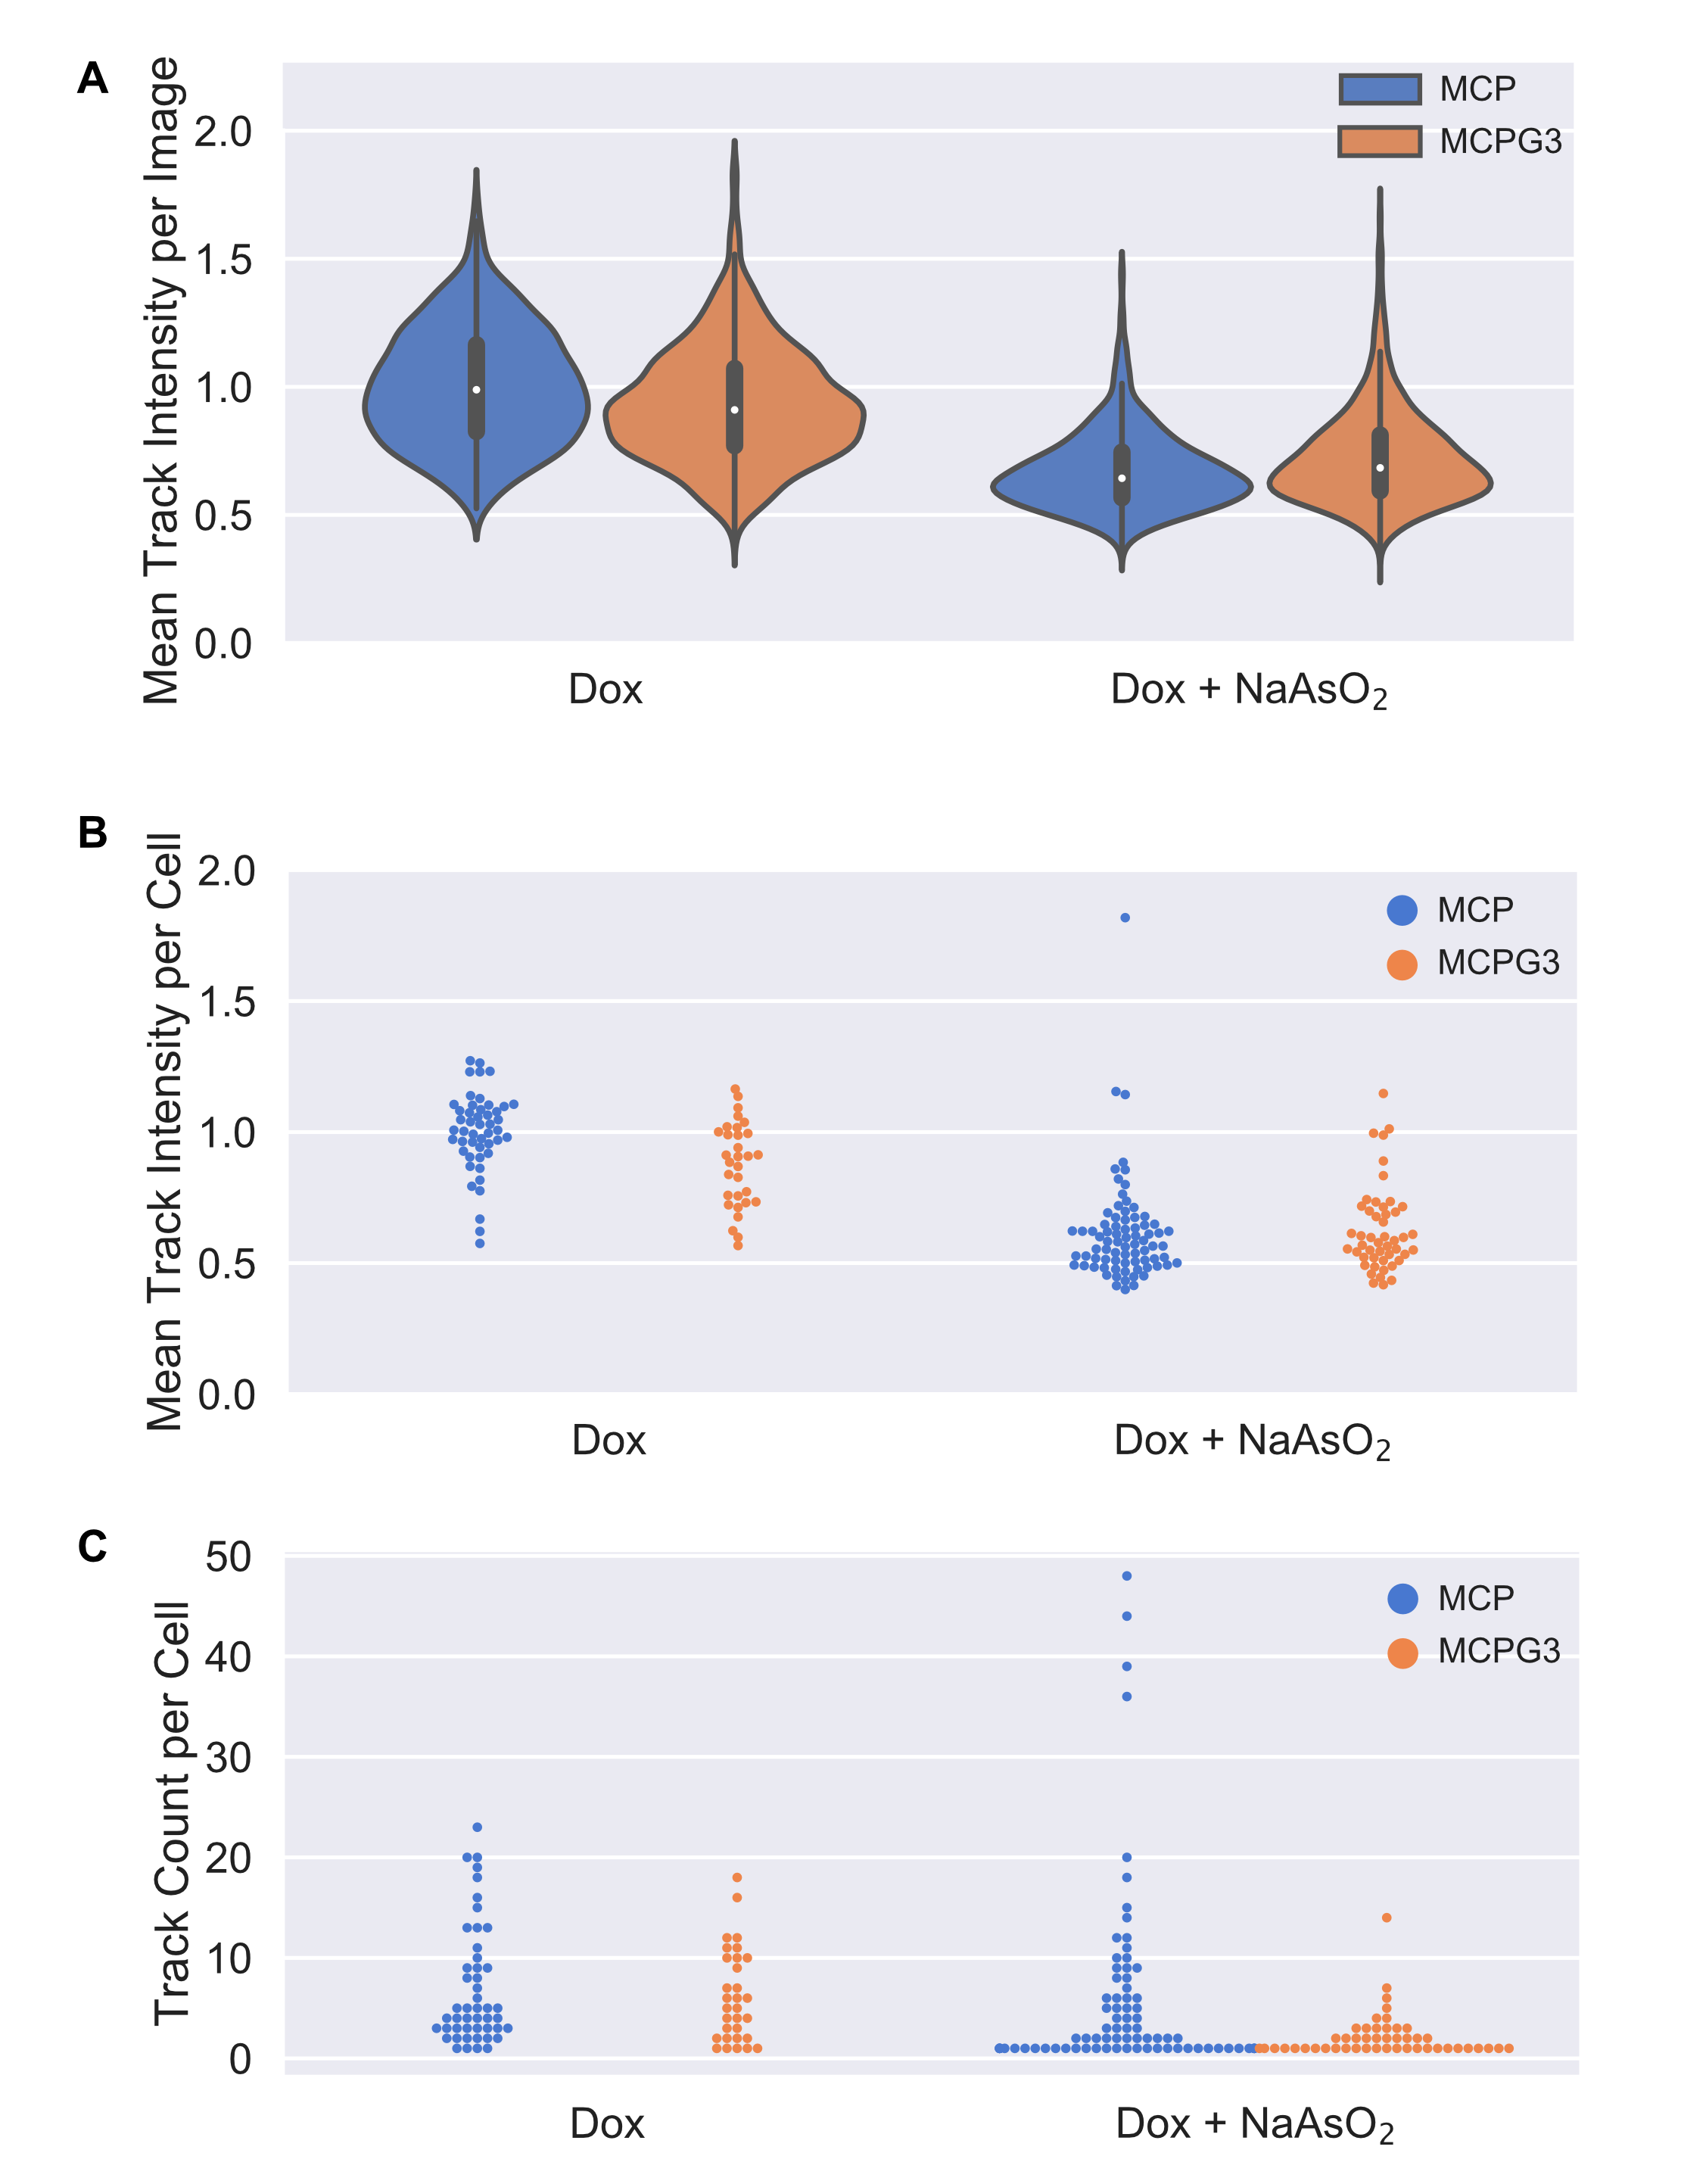
\includegraphics[width=\linewidth]{images/figure4}
    \caption{(On the previous page.)}
    \label{fig:mcp_suntag}
\end{figure}


\subsection{Transcript stability is affected by G3BP1 tethering} \label{mcp_treat}

SunTag measurements (see Section \ref{mcp_suntag}) did not suggest any effect of G3BP1 on translational activity.
Alternatively, a decrease in mRNA degradation could also explain the original luciferase readings.
To ask whether G3BP1 has an mRNA stabilizing effect, I compared the number of intact transcripts between MCPG3 and the control using 3(three)'-RNA end accumulation during turnover (TREAT) \cite{horvathova_dynamics_2017}.

TREAT uses a slightly modified reporter mRNA containing viral RNA pseudo-knot (PK) structures upstream of the MS2 stem-loops.
These PKs can block Xrn1 mediated 5'-3' degradation of a transcript by sequestering the 5' phosphate group \cite{kieft_new_2015}.
Subsequently, by using FISH probes against \textit{Renilla} luciferase upstream of PKs (showing intact mRNAs) and FISH probes against MS2 stem-loops downstream of PKs (showing both intact and degraded mRNAs) one can quantify the number of intact transcripts.

To look at transcript stabilization, a cell line expressing the aforementioned TREAT mRNA reporter was used.
Five time points were chosen after a 1 hour induction followed by thorough washing to halt any further transcription.
As can be seen in Figure \ref{fig:mcp_treat}A, transcripts get exported to the cytosol as soon as transcription is stopped.

When comparing the percentage of intact mRNAs, i.e. transcripts still containing FISH spots against both \textit{Renilla} luciferase and MS2, between MCPG3 and the control, a striking difference is evident (Figure \ref{fig:mcp_treat}B).
The G3BP1 fusion shows a significant reduction in degraded transcripts compared to the control suggesting an increase in mRNA stability.
This effect is not reflected in the mRNA count from the SunTag measurements (see Section \ref{mcp_suntag}) which might arise from the nature of the SunTag cassette that will be discussed in the following Section \ref{spaghetti}.


\begin{figure}[h]
    \centering
    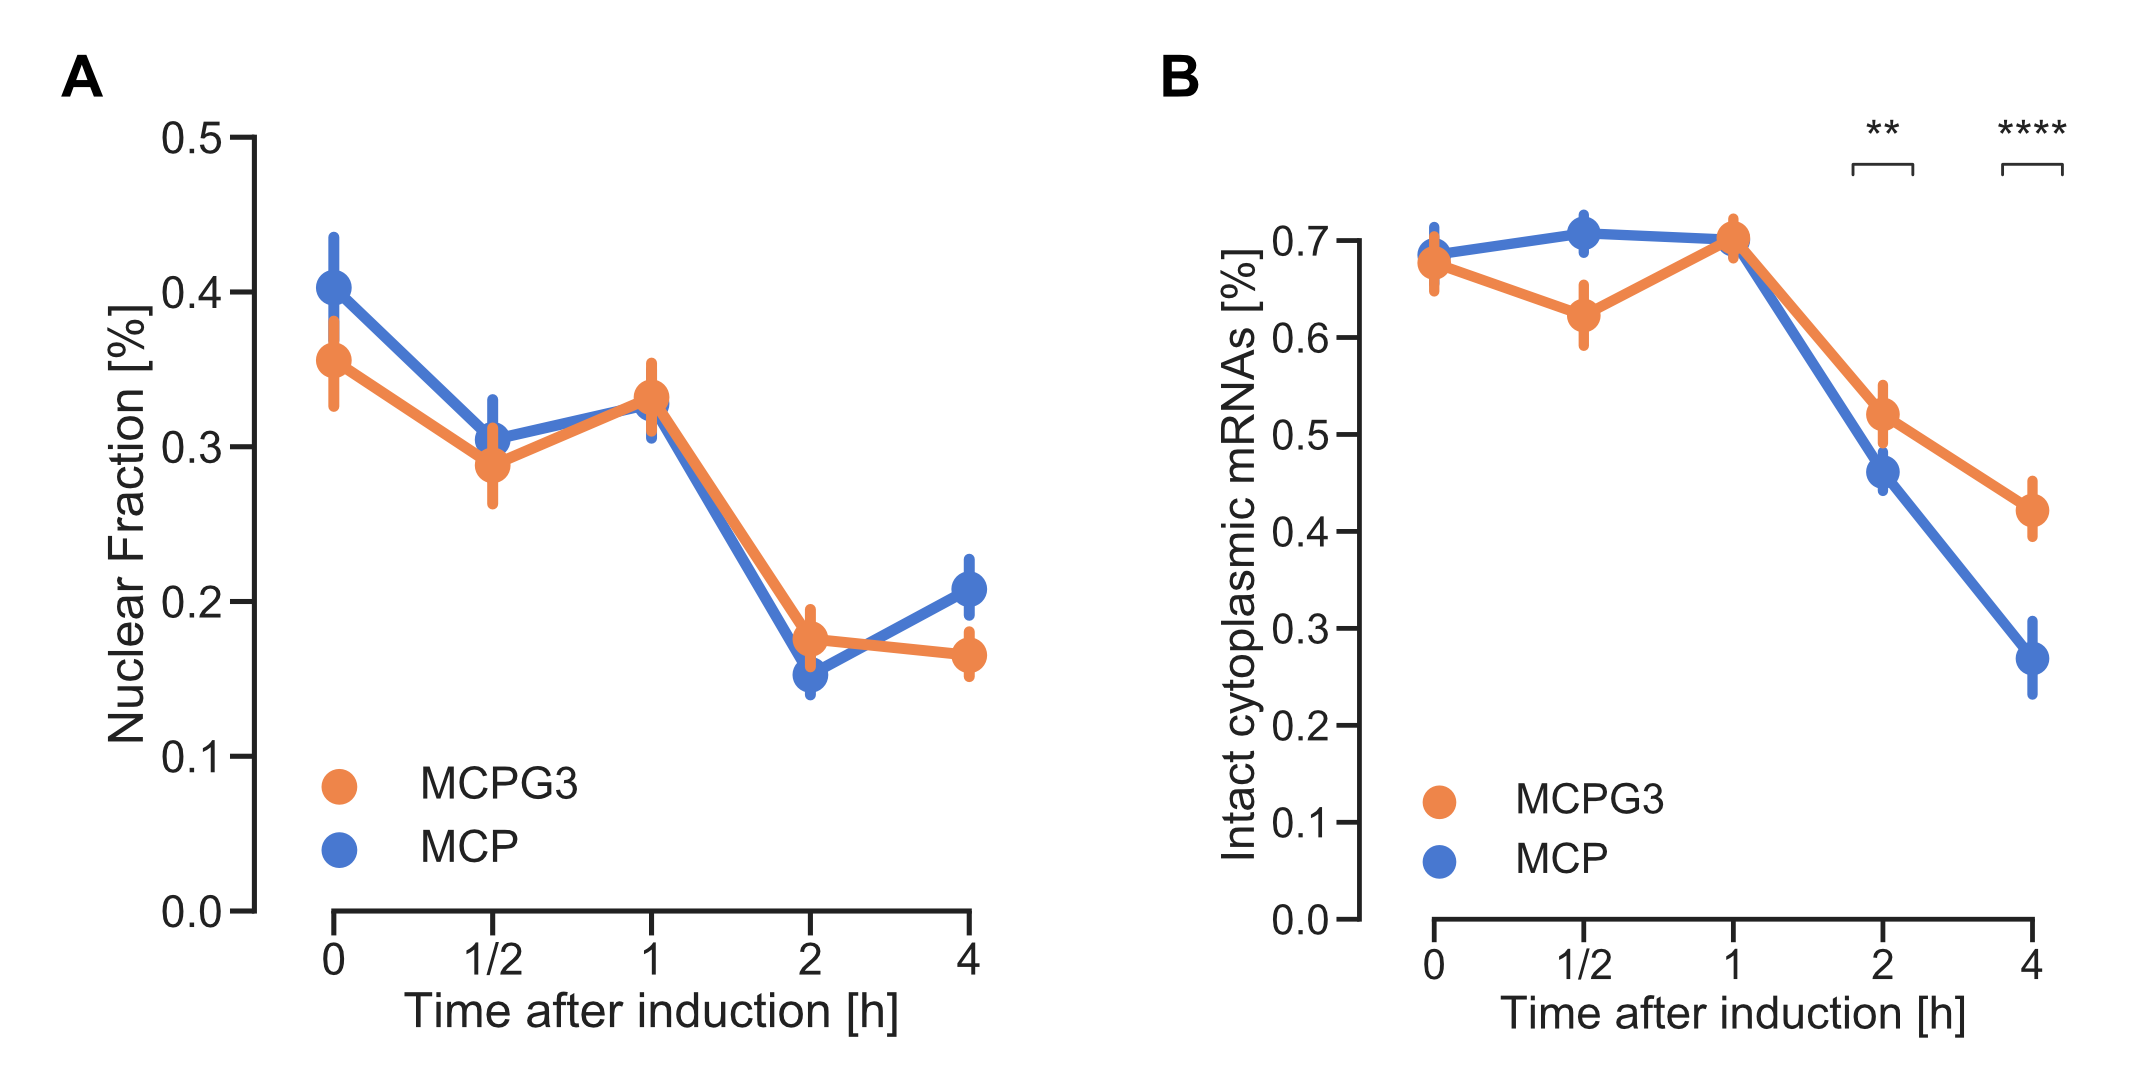
\includegraphics[width=\linewidth]{images/figure5}
    \caption{\textbf{TREAT based mRNA stability assay.}
        (A) The fraction of nuclear mRNAs (of total cellular mRNAs)
            at different time points after induction.
        (B) Percentage of intact cytoplasmic mRNAs at different time points.
        (A and B) Number of cells quantified (ascending, MCP then MCPG3):
            117, 154, 200, 175, 55, 114, 148, 167, 111, 132.
    }
    \label{fig:mcp_treat}
\end{figure}


\section{How can the SunTag reporter be improved?} \label{spaghetti}

The original design of the SunTag cassette consists of 24 GCN4 repeats.
These completely disordered repeats are thought to aggregate and could lead to a decrease in translation rates \cite{gurry_order_2015}.
In an attempt to decrease protein disorder, a spaghetti monster reporter was made \cite{zhao_genetically_2019}.
Spaghetti monster green fluorescent proteins (smGFP) are essentially a non-fluorescent green fluorescent protein's (GFP) beta-barrel used to attach small epitope tags.
Here, three GCN4 repeats each were placed at the N-terminus, C-terminus, and 10/11-loop of the GFP beta-barrel as shown in Figure \ref{fig:spaghetti}A.
Previously, other tags, such as influenza hemagglutinin (HA), were used and visualized with frankenbodies (single-chain antibodies targeting various tags).
In this study, I attempt to combine SunTag imaging with smGFP constructs.

Initially, it was of interest to see whether the smGFP reporter has higher translational activity.
As is evident from Figure \ref{fig:spaghetti}B, the new reporter shows an approximative 4-fold increase in luciferase activity compared to the original SunTag reporter.
A pure \textit{Renilla} reporter was used as control which does not contain any GCN4 repeats.
While the smGFP reporter drastically increases activity, it does not yet reach the levels of the control.
It must be noted, that the control construct does not contain an FKBP tag which has lowered the luciferase activity in previous experiments by enhancing the degradation of the tagged protein \cite{bonger_small_2011}.

To look at the effect of the new reporter in live cells, stable cell lines were created and observed after 1 hour of induction.
From a representative image in Figure \ref{fig:spaghetti}C, one can see that cells typically have more, slightly dimmer translation sites.
Quantification of images showed a significant increase in the number of translation sites per cell compared to the cells expressing the standard SunTag reporter (Figure \ref{fig:spaghetti}D).
The brightness of individual spots decreased around 2.7 fold (Figure \ref{fig:spaghetti}E).
This decrease can be explained by a lower number of GCN4 repeats available for the scAB to bind.
Whereas the standard SunTag has 24 GCN4 repeats, smGFP only has 9 leading to a binding site difference of 2.6$\overline{\mbox{6}}$ to 1.

Taken together, this study proposes a new SunTag reporter which increases translational activity by greatly increasing the number of active transcription sites.
This new reporter allows for shorter induction times and the folded structure should reduce aggregation-based problems.


\begin{figure}[h]
    \centering
    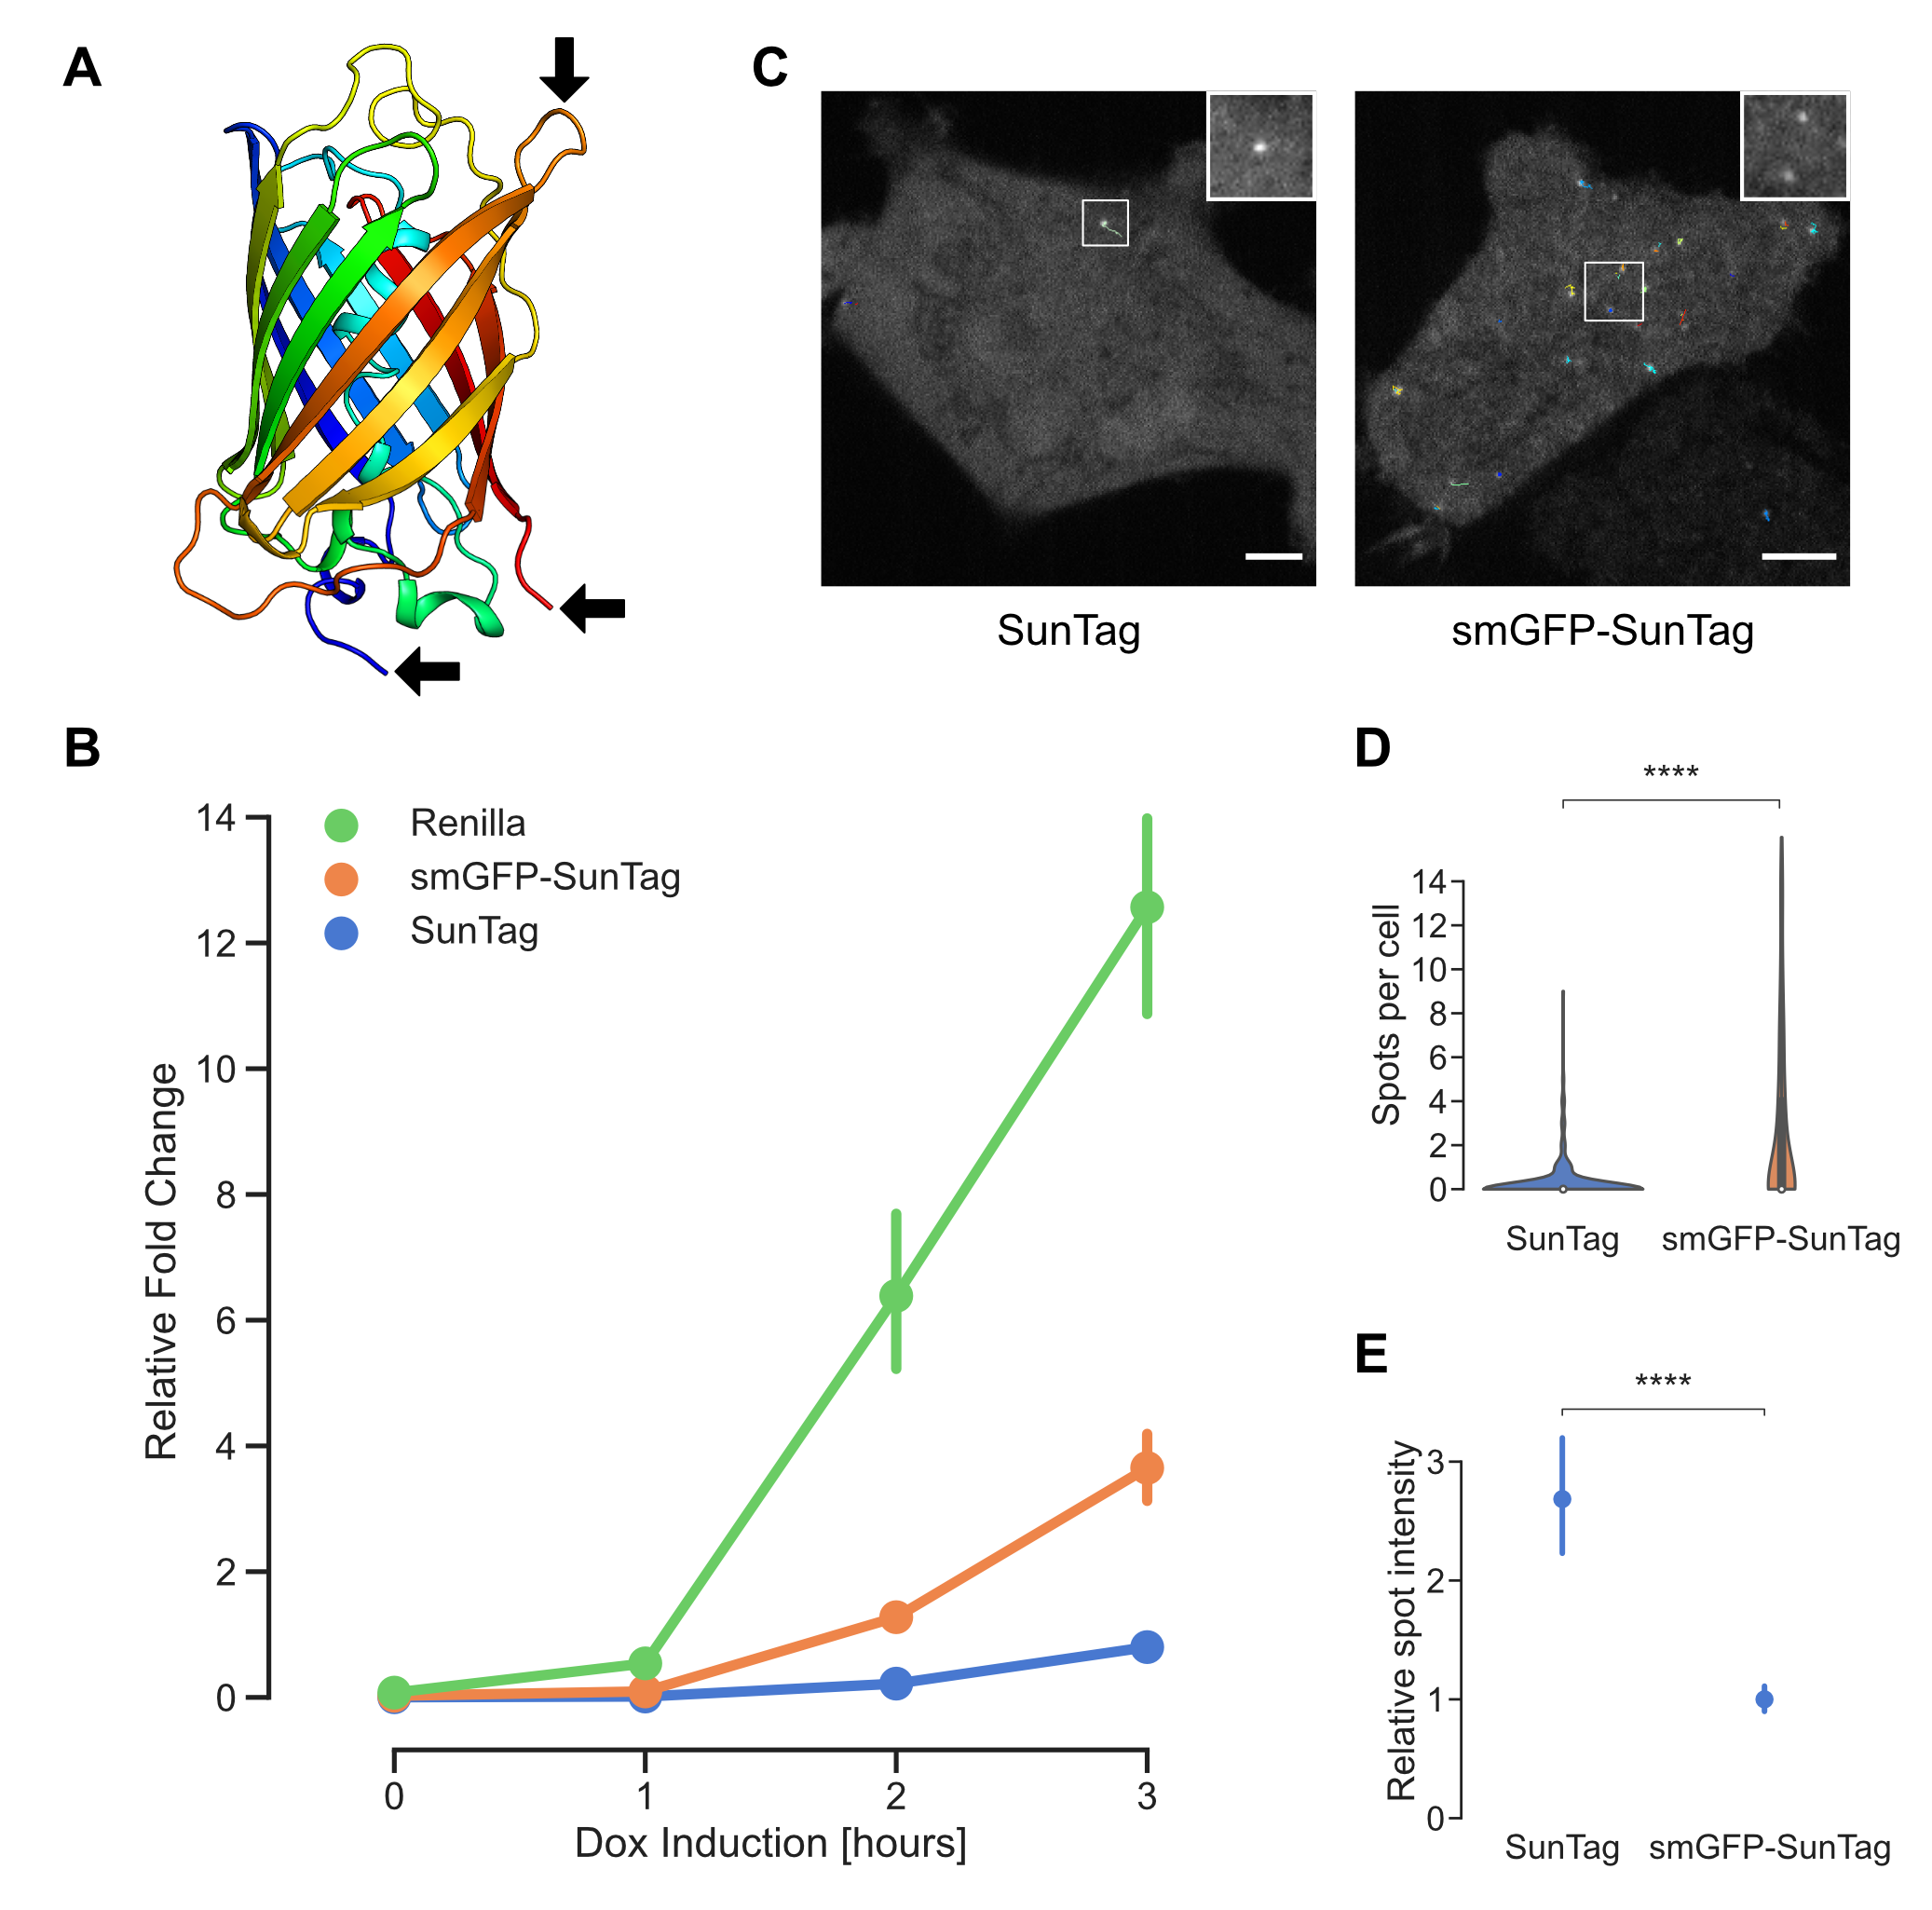
\includegraphics[width=\linewidth]{images/figure6}
    \caption{\textbf{Overview of the smGFP SunTag reporter.}
        (A) Structural overview of GCN4 repeat placement on the smGFP beta-barrel (PDB ID: 1GFL \cite{yang_molecular_1996}).
        (B) Relative luciferase activity comparing the standard SunTag reporter,
            the smGFP SunTag reporter, and a Renilla reporter without SunTag cassette.
        (C) Representative fluorescence images. Each recorded mRNA track is 
            visualized with a unique color. Scale bar, 10 \textmu m.
            The inset shows spots from raw images without brightness corrections.
        (D) Quantification of translation site count per cell.
            The number of cells quantified (left to right): 286, 233.
        (E) Average spot intensity normalized to the smGFP reporter.
            The number of spots quantified (left to right): 36, 39.
    }
    \label{fig:spaghetti}
\end{figure}